\section{Evaluation}
\label{sec:evaluation}
The consideration of usability about Recluse is time cost in each authentication. However, the Recluse also introduces the extra storage as IdP and RP has to remember the longer identifier of user and RP. But the storage cost is within the range of TBs, which is to be ignored.

\subsection{Settings}
The prototype of Recluse has been implementation on the system consisting of 3 computers.
The IdP is on the DELL OptiPlex 9020 PC with an Intel Core i7-4770 CPU, 500GB SSD and 8GB of RAM running Window 10 pro. The RP is on the ThinkCentre M9350z-D109 PC with an Intel Core i7-4770s CPU, 128GB SSD and 8GB of RAM running Window 10 pro. The user agent is on the Acer VN7-591G-51SS Laptop with an Intel Core i5-4210H CPU, 128GB SSD and 8GB of RAM running Windows 10 pro.
The system is linked through the D-Link DGS-1008D Unmanaged Gigabit Ethernet Switch.

Additionally, the version of Chrome is 75.0.3770.100, and the version of Spring framework is 2.0.5.

The timer starts when the user click the login button and stops while the RP identifies the user. To run the login process automatically, the JavaScript code is inserted to the RP's web page to simulate the clicking the login button.

\subsection{Result}
We run the authentication on Recluse prototype system 1000 times and get the average time of the whole authentication flow is 210 ms. Compared with the traditional OIDC system, Recluse introduces the RP identifier transforming and dynamic registration, the average time cost of which are 49 ms and 42 ms. Additionally, Recluse also change the the generation of $RPID_T$ and $PPID$, which introduces extra Modular Exponentiation and Extended Euclidean computation. It is inspected that the Modular Exponentiation computation in $RPID_T$ generating conducted by RP and user agent cost 3 ms and 10 ms, the computation conducted by IdP while generating $PPID$ costs 2 ms, as the power in the above computations are not longer than 256 bits. While RP identifies the user, the trapdoor $t$ is generated by the Extended Euclidean algorithm, which costs 3 ms in average. Then RP derives the $Account$ from $PPID$ by the Modular Exponentiation computation the power of which is $t$ no longer than 2048 bits, costing 54 ms in average.
%, in which the Negotiation costs 309 ms , the Dynamic Registration costs 129 ms, and the Authentication costs 107 ms.

%The most time cost is introduced by the modular power and extended euclidean operation. It is evaluated that the time cost of each modular power operation in RP, user agent and IdP are about 30 ms, 100 ms and 30 ms. During the login flow contains modular power operation is conducted 4 times by RP, 3 times by user agent and 1 time by IdP.


\subsection{Comparison}
We also run the unmodified MITREid Connect and SPRESSO (with the open-source project) system with the similar timer and automated scripts to see the comparison.
It is inspected that the time cost of MITREid Connect and SPRESSO are 69 ms and 295 ms at best. To compare Recluse with MITREid Connect and SPRESSO in detail, we formally split the authentication process in the SSO systems into specific phases,
\begin{itemize}
    \item  Authentication request initiated, which starts when the user agent sends the login request to RP and ends while IdP receives the authentication request.
    \item  Identify proof generated, the phase IdP generates the identity proof after receiving the authentication request.
    \item  Identity proof transmitted, from IdP sending the identity proof to RP receiving the Identity proof.
    \item  Identity proof verified, the phase RP identifies the user through the identity proof.
\end{itemize}

\begin{figure}
  \centering
  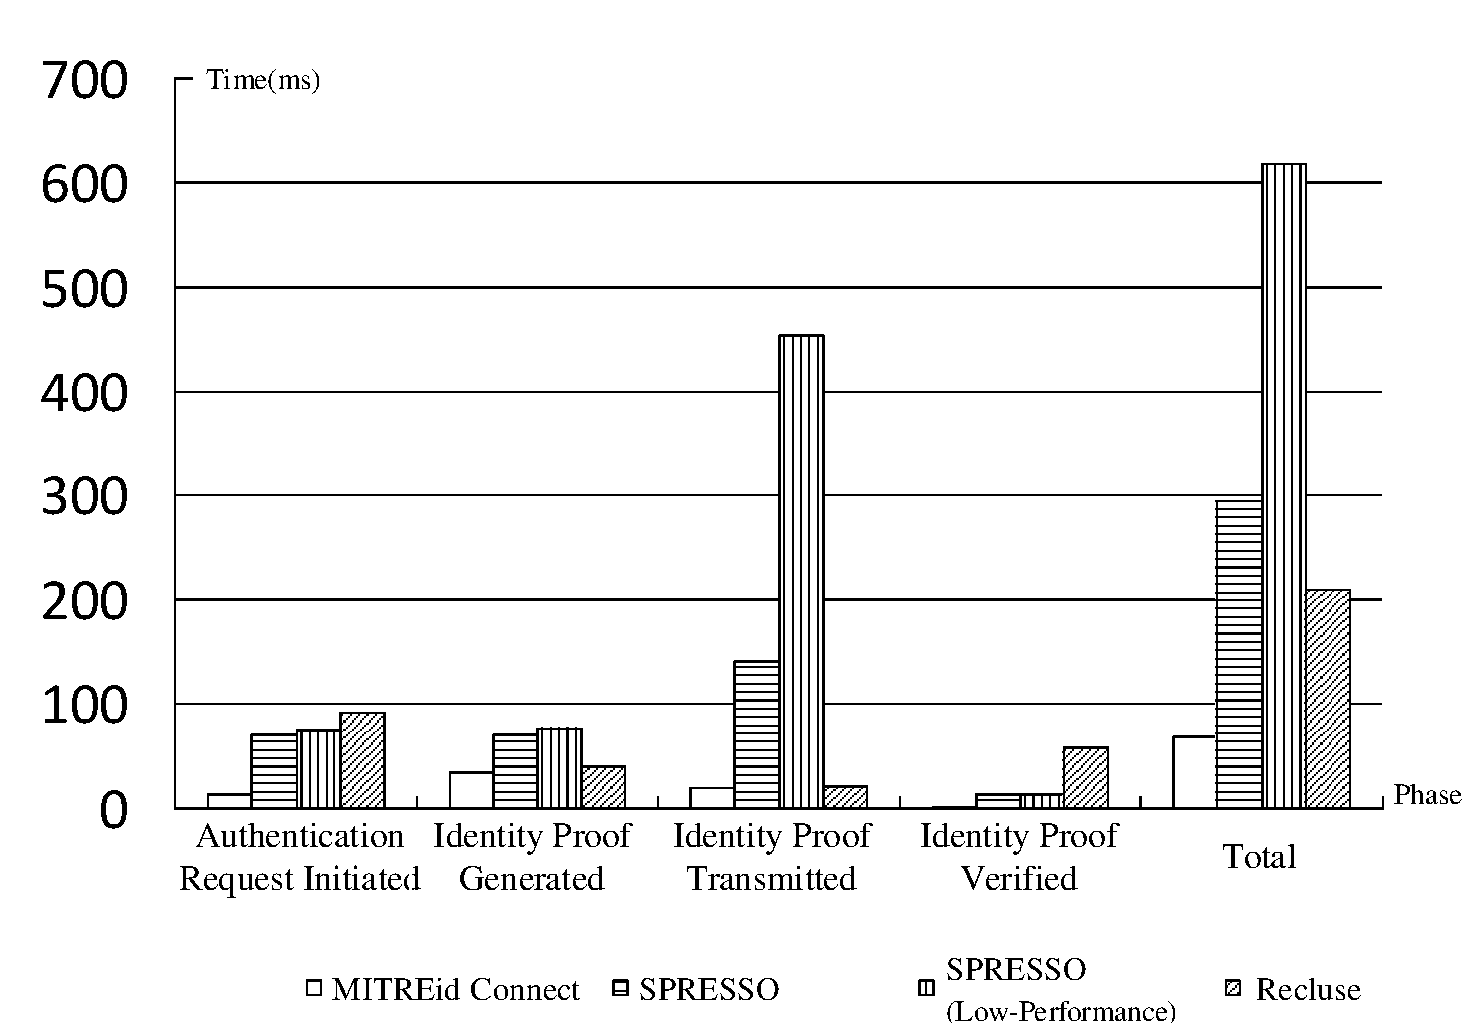
\includegraphics[width=\linewidth]{fig/evaluation.pdf}
  %\subfigure[Authorization Code Flow]{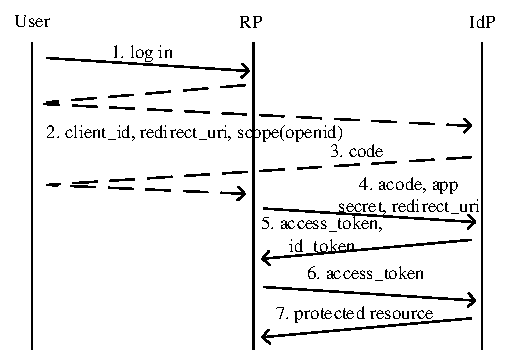
\includegraphics[width=\linewidth]{fig/openidconnect2.pdf}\label{fig:OpenID_code}}
  %\subfigure[Hybrid Flow]{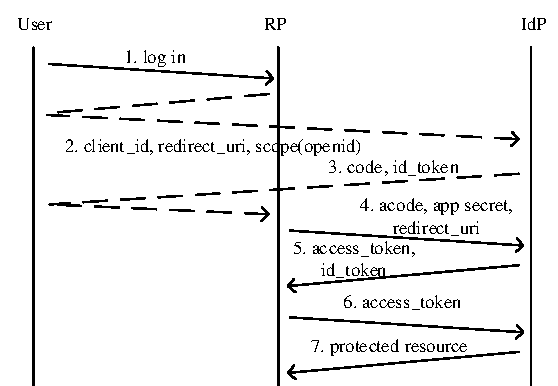
\includegraphics[width=\linewidth]{fig/openidconnect3.pdf}\label{fig:OpenID_hybrid}}
  \caption{The Evaluation.}
  \label{fig:evaluation}
\end{figure}
The comparison of Recluse, MITREid Connect and SPRESSO is shown as Figure~\ref{fig:evaluation}.

In the authentication request initiated phase, MITREid Connect uses the shortest time, 13 ms, as it only builds the request with the stored parameters, such as \verb+client_id+ and \verb+redirect_uri+. SPRESSO introduces the additional request from RP to IdP for IdP's public parameters and the encryption operation to generate \verb+tag+ (the encrypted RP identifier), so that the time cost is 71 ms. Recluse use the longest time, 91 ms , which introduces the extra negotiation and dynamic registration in this phase including 1 time Modular Exponentiation computations at user agent and 2 Modular Exponentiation computations at RP.

In the phase of identity proof generated, all of the systems offer the signed identity proof. Compared with MITREid Connect, Recluse only introduces the extra Modular Exponentiation computation for $PPID$. However, the SPRESSO provides the totally different format of identity proof. The time cost in this phase of MITREid Connect, SPRESSO and Recluse are 35 ms, 71 ms and 40 ms.

In the phase of identity proof transmitted, Recluse transmits the identity proof through the extension and the MITREid Connect uses JavaScript code in RP's web page , the time cost of which are 21 ms and 20 ms. The SPRESSO requires the additional opened iframe, which downloads the script from FWD for extra encryption and decryption operation for identity proof transmitted. However, the time cost of these operations are significant different while running user agent in different devices. We get the 140 ms in average at best, however, in another low-performance device, the number is 453 ms. To verify whether the performance of user agent has the same influence on Recluse, we use several PCs to log in Recluse and record the time. The result is the time costs in these PCs are quite similar which means the performance of user agent is not apparently influential with Recluse.

The identity proof verified at RP only costs about 1 ms for signature verifying, which is 58 ms at RP requiring additional Modular Exponentiation and Extended Euclidean computation. The RP of SPRESSO has to decrypt the identity proof and verify the signature, which costs 13 ms.

In conclusion, compared with MITREid Connect, Recluse introduces about 135 ms extra time cost in authentication request initiated and identity proof verified, which is acceptable. Compared with the best result of SPRESSO, Recluse still saves 85 ms.

%We also evaluate the time cost of traditional MITREid connect system in the same circumstance, which is about 130 ms. And the time cost of SPRESSO is about 400 ms.
%Therefore, the time cost of Recluse is acceptable.


\begin{comment}
The prototype system runs on Thinkcentre M8600t with an Intel Core i7-6700 CPU, 500GB SSD and 8GB of RAM running Windows 10.
\subsection{Implementation}
%与原系统相比做了哪些改动
Implementation of system contains modification of IdP as well as RP and creation of user agent. User agent runs on chrome 71.0.3578.98 as its extension.

System's parameters are carefully chosen in specification about \textbf{Difie-Hellman} algorithm. $p$ is one of primes provided by the specification and $a$ is its generator. All the primitive elements module $p$ is generated by $a$.

Compared with formal openid connect system, the work we do is shown as following:
\begin{itemize}
    \item Modifying RP registration so that IdP is able to offer RP\_cert to RP.
    \item Providing RP's client\_id negotiation interface.
    \item Providing RP's dynamic registration acceptance interface.
    \item Implementing user-id-generating algorithm at IdP.
    \item Implementing the function of getting user\_rp\_id from user\_id at RP.
    \item Realizing function of client\_id negotiation, dynamic registration, id\_token transmitting and so on at user agent.
\end{itemize}
\subsection{Storage}
As the prime $p$ is 2048-bit-length, storage of client\_id, user\_id and user\_rp\_id are no larger than 512 Bytes as hexadecimal. We consider they are all 512 Bytes in evaluation.

For IdP and RP's user Personally Identifiable Information (PII) storage, it changes from a short user id into a 512 Bytes id. It is assumed that an IdP owns 100 million users and an RP owns 10 million users. If a user's PII costs 500 Bytes extra storage so that IdP need to offer 50 billion Bytes (less than 50 GB) storage and RP need to offer 5 billion Bytes (less than 5 GB) storage. The extra cost of storage can be omitted.

For IdP's dynamic registration storage, the data contains RP's client\_id and redirect\_uri. We consider that each dynamic registration data cost no more than 550 Bytes storage. And for each client\_id IdP can set the lifetime of validity. It is assumed that for each client\_id its lifetime is 2 minutes and during 2 minutes there are 1 million requests for dynamic registration. So IdP need to offer 550 million Bytes (about 500 MB) storage for dynamic registration. The extra cost of storage can be omitted.

For user's login log stored in RP and IdP, RP and IdP are able to transform PII into a shorter hash characters. So it almost cost no more extra storage.
\subsection{Timings}
Table~\ref{tab:timeings} shows the result of the time cost in PRISSO's each phases. We log in the prototype 100 times and figure out the average time cost. It can be found that the most of time consumed in client\_id negotiation phase, dynamic registration conducted by user and IdP providing id\_token. They cost 4337ms in average which is more than 90\% of total time. In client\_id negotiation to confirm $r=pk\_rp^y mod p$ is a relative prime of $p-1$ user has to continue generating $y$ until $r$ is validate which costs most of time. In dynamic registration user need check validation of basic\_rp\_id and IdP's URL by rp\_certificate, calculate client\_id by basic\_rp\_id, $r$ and check the result of registration and forward it to RP. In SSO system if user firstly log in an RP it is necessary for user to confirm permission of login in the specific RP. It is showed as user has to press the confirm button in IdP's website. In PRISSO client\_id is random so that every login for a user is first login. So every login requires user to press a button redundantly. Even the press action is conducted by chrome extension, it costs some time.

We also do login in traditional OpenID-Connect system 100 times and get a total time cost 44ms in average. Compared with traditional system, PRISSO's time cost is about 100 times.
\begin{table}
\caption{Benchmark Result}
\begin{tabular*}{\linewidth}{@{\extracolsep{\fill}}ll}
\toprule
phase& time (ms)\\
\hline
Client\_id Negotiation (RP)& 49\\
Client\_id Negotiation (user)& 2967\\
Dynamic registration (IdP)& 16\\
Dynamic registration (user)& 1001\\
Obtaining Token (IdP)& 369\\
Obtaining Token (RP)& 19\\
Network Cost& 12\\
Total Time& 4433\\
\bottomrule
\label{tab:timeings}
\end{tabular*}
\end{table}
%\subsection{Throughput}

\subsection{Optimizing}
As the most time cost is in client\_id negotiation and dynamic registration and these two phases are transparent to user. To reduce time cost we move client\_id negotiation and dynamic registration to website initiation. When user visit RP's login page user agent conducts client\_id negotiation and dynamic registration during page loading. So for a user its login procedure starts at obtaining token and network time cost is halved. The total time cost is about 406ms and the system possesses practicability.
\end{comment}
